%!TEX root = ..\main.tex
\section{Model}
\label{sec:model}

\begin{figure*}[t]
\centering
	
\includegraphics[width=0.9\textwidth]{Images/fullSystemPicture}
	\captionsetup{justification=centering, width=0.9\textwidth}
	\caption{Snapshot obtained from Langevin dynamics simulations for density $\rho = 0.95$ and $k_BT = 1.5$. The arrows represent the dipole moment of the particle. The simulation was allowed to equilibrate for time $t = 100$.}
	\label{fig:fullSystemPicture}
\end{figure*}

We consider colloidal particles with a permanent dipole moment $\mu \hat{m}$, where $\hat{m}$ is a unitary vector along the direction of the dipole moment. While considering a three-dimensional system, we constrain particle translational motion to a one-dimensional line, i.e. particles are confined to the $z$ axis. However, particles can explore the full three-dimensional orientation space. A snapshot of the system is shown in the \figref{fig:fullSystemPicture}.

The particle-particle interaction is described as the superposition of two contributions: a dipole-dipole interaction and a short-range repulsion.

The energy of dipole-dipole pairwise interaction between particles $i$ and $j$ is

\begin{equation}
\label{eq:dipole_dipole_interaction}
U^{dip}_{ij} =
	- \frac{\mu_i \mu_j}{\Delta r^3}[
		3 (\hat{m}_i \cdot \hat{r}_{ij})(\hat{m}_j \cdot \hat{r}_{ij})
		- (\hat{m}_i \cdot \hat{m}_j)
	]
\end{equation}
where $\mu_i \hat{m}_i$ and $\mu_j \hat{m}_j$ are dipole moments of interacting particles, $\boldsymbol{r}_{ij}$ is the vector which connecting the center of both particles, and $\Delta r$ is the absolute value of the distance the center of the particles.

Since the position of the particles is constrained to a line along the z axis, $\boldsymbol{r}_{ij}$ is always along with $z$ axis. Assuming that all particles have the same dipole moment $\mu_i = \mu_j \equiv \mu$, and defining $\mu = 1$, Eq. \eqref{eq:dipole_dipole_interaction} can be simplified as,

\begin{equation}
\label{eq:dipole_dipole_1D}
U_{ij}^{dip} = - \frac{1}{\Delta z^3} [3 \cos \theta_i \cos \theta_j - (\hat{m}_i \cdot \hat{m}_j)]
\end{equation}
where $\theta_i$ and $\theta_j$ are the angles between $z$ axis and dipole moments of particles $i$ and $j$, respectively, and $\Delta z = |z_j - z_i|$, where $z_i$ and $z_j$ are particle positions along the $z$ axis.

The repulsive part is described by Yukawa potential
\begin{equation}
\label{eq:yukawa_interaction}
U_{ij}^{rep} = \frac{A \exp(-k \Delta z)}{\Delta z},
\end{equation}
where $A$ and $k^{-1}$ are the strength and range of interaction. 

In this work we define thermal energy $k_BT$ in units of dipole-dipole interaction potential, (i.e. $k_BT = \epsilon \mu^2$, where $\epsilon$ is reduced energy), and maintain the ratio between $\mu$ and $A$ as constant. Without loss of generality, we can define $\mu = 1$.

\begin{figure}[p]
\centering
	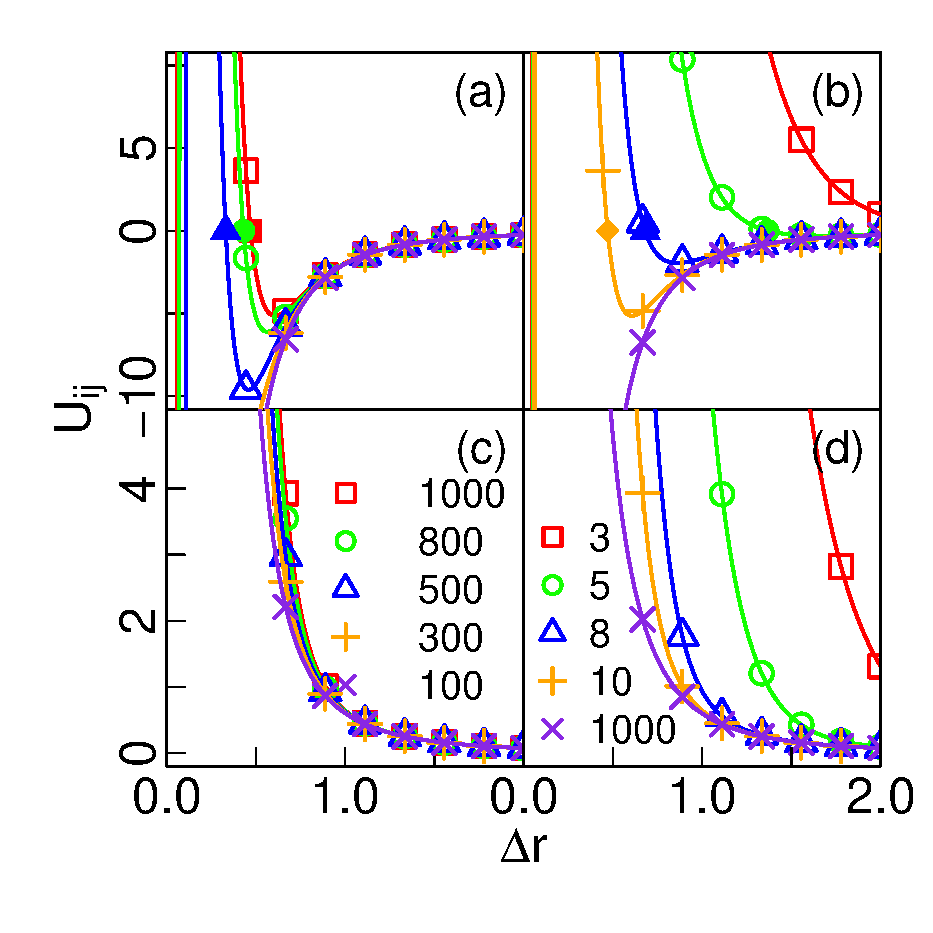
\includegraphics[width=0.9\textwidth]{Images/particle_interaction_potential}
\captionsetup{justification=centering, width=0.9\textwidth}
\caption{Energy of the pairwise interaction as function of the interparticle distance when both dipoles are aligned (top) or one is perpendicular (bottom) to the $z$ axis. For the plots a) and c) we fix the interparticle distance when the dipoles are for $k = 10$, and for b) and d) we fix for $A = 1000$.}
\label{fig:interaction_energy}
\end{figure}

When the dipole moments are perpendicular to each other, the interaction is purely repulsive for any given $A$ and $k$. However, as we can see on the Figs.~\ref{fig:interaction_energy}(a)~and~(b), for co-aligned configurations for significantly low values of $A$ and high values of $k$, the interaction is purely attractive. We will not consider those cases, as the system will be unstable and all particles will coalesce into one point. In this work, to reduce the number of free parameters we fix $A = 1000 \mu$ and $k = 10$.
